
\chapter{算法实现}

\section{图像预处理}

受光照条件和噪声等因素的影响,图像的质量不佳,不能直接用于数字识别。需要进行预处理,改善图像质量,从而更容易识别数字。本文采用的预处理方法有\emph{灰度化},\emph{高斯滤波}和\emph{直方图均衡}。

\subsection{灰度化}



摄像头采集的图像是彩色图像,如图\ref{fig:src}所示。由于待识别的数字在右上角,所以只需截取右上部分做后续处理,如图\ref{fig:rgb}所示。首先将彩色图像转换成灰度图像。这样做的原因是:
\begin{asparaenum}[(1)]
\item 灰度图像只有一个分量,比三分量的彩色图像更易处理;
\item 本文识别的数字边框为黑底白字,边框内绝大部分像素都是黑白颜色,灰度化后颜色基本没有变化。
\end{asparaenum}

本文使用加权平均法求出灰度图像,公式为$I=0.114R+0.587G+0.299B$。灰度图像如\ref{fig:gray}所示。
\begin{figure}[h]
  \centering
  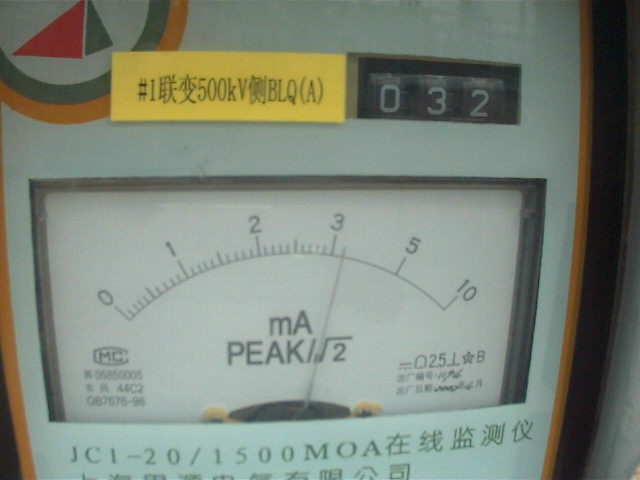
\includegraphics[scale=0.5]{src.png}
  \caption{原始图像}
  \label{fig:src}
\end{figure}
\begin{figure}[h]
  \centering
  \subfloat[彩色图像]{\label{fig:rgb}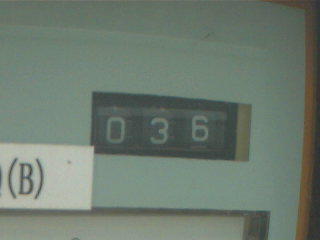
\includegraphics[scale=0.5]{rgb.png}}\hspace{1in}
  \subfloat[灰度图像]{\label{fig:gray}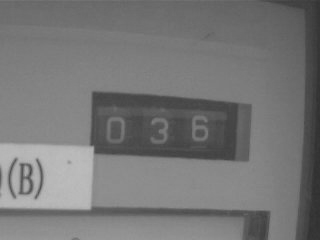
\includegraphics[scale=0.5]{gray.png}}
  \caption{灰度化}
\end{figure}

\subsection{高斯滤波}


灰度图像含有较多噪声,不利于提取目标,需要用图像平滑的方法减少噪声。观察发现,待处理图像的噪声以盐椒噪声为主,因此选用高斯滤波进行平滑滤波。在调用OpenCV的高斯滤波函数时,要指定高斯滤波模板的长宽,$\sigma$值和边界扩充类型。一般情况下,只需使用长宽相等的高斯滤波模板。模板尺寸越大,平滑的效果越好,但图像的边缘也越模糊。综合以上情况,将长和宽均设置为3。$\sigma$值的设定也有一定的要求。高斯函数在半径为$2\sigma$范围内的积分为0.95,故绝大部分权值集中在这个领域内。为了最大限度地发挥高斯滤波的效果,需要保证模板能覆盖这个邻域,即$m\sigma$。边界扩充类型指将高斯滤波模板中心与图像边界重合,模板覆盖的部分像素超出图像边界时,这部分像素值的计算方式。一般的做法是将边界内的像素值复制到边界外。高斯滤波的效果如\ref{fig:gauss}所示。
\begin{figure}[h]
  \centering
  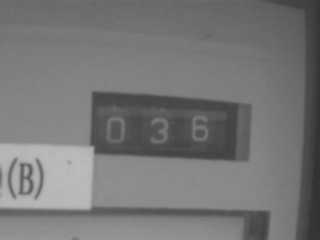
\includegraphics[scale=0.5]{gaussian.png}
  \caption{高斯滤波}
  \label{fig:gauss}
\end{figure}

\subsection{直方图均衡}


由于不同时间内光照条件不同,不同时间采集的图像的整体亮度不同。例如日光微弱时图像整体偏暗,日光强烈时图像整体偏亮。偏暗和偏亮的图像对比度不高,不利于识别。因此,采用直方图均衡化的方法增强图像的动态范围,从而达到增强图像整体对比度的效果。实验发现,在进行直方图均衡化前,需要进行图像平滑。这是因为直方图均衡对图像的所有像素的灰度不加选择地加以扩充,因此噪声的灰度也被扩充,使原本灰度相近的区域灰度差距加大,对图像分割造成不利影响。

比较均衡化前的直方图\ref{fig:histsrc}和均衡化后的直方图\ref{fig:histequal}分别是均衡化前和均衡化后的直方图,可以发现均衡化后的直方图比均衡化前的直方图具有更宽的动态范围,每个灰度级上有大致相等的像素数。
\begin{figure}[h]
  \centering
  \subfloat[均衡化前的直方图]{\label{fig:histsrc}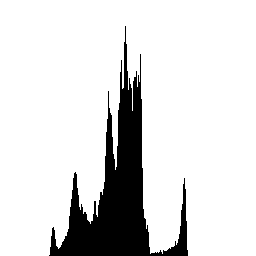
\includegraphics[scale=0.5]{histsrc.png}}
  \subfloat[均衡化后的直方图]{\label{fig:histequal}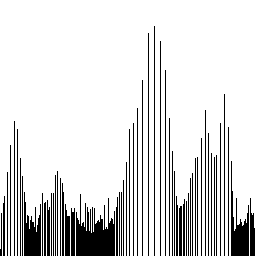
\includegraphics[scale=0.5]{histequal.png}}
  \caption{均衡化前后的直方图}
\end{figure}
直方图均衡化后的图像如图\ref{fig:equal}所示。经直方图均衡化后,不同时间的图像灰度分布大致相同,对于图像分割和识别是十分有益的。
\begin{figure}[h]
  \centering
  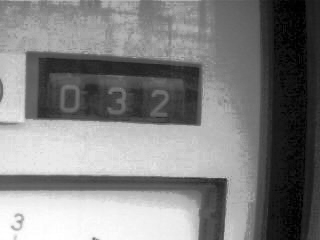
\includegraphics[scale=0.5]{equal.png}
  \caption{直方图均衡化}
  \label{fig:equal}
\end{figure}



\section{数字边框定位}

数字边框定位是电表读数识别的一个关键环节,也是较难的环节。数字边框内的数字是待识别的目标,数字边框外的图像则为无用信息。直接从原图中提取数字,难度大,准确率低。因此,应首先找出数字边框,去除无用的部分。观察图\ref{fig:equal}发现,数字边框周围有一些干扰区域,如右侧的电表边框和下侧的指针边框颜色灰度和数字边框的背景类似。这些干扰区域增加了分割的难度。

\section{二值化}

数字边框定位的第一步是二值化,即将原图分割为目标区域和背景区域,将目标区域的灰度设为255,背景区域的灰度设为0。分割的关键是找到阈值,将高于阈值和低于阈值的像素划分到两个区域中。所有由于本文的灰度图像由大片的黑色和白色区域组成,可以使用Otsu算法分割阈值。




\section{数字分割}

目前没有一种通用的分割方法,适用于各个领域。应该根据实际情况和领域知识,灵活地选定一种方案。

\section{数字识别}



%%% Local Variables: 
%%% mode: latex
%%% TeX-master: "thesis"
%%% End: 
